% !TeX program = lualatex
\documentclass[tikz,multi=tikzpicture,border=7pt]{standalone}

\usepackage{amsmath}
\usepackage{newcomputermodern}
\usepackage{xcolor}
\usetikzlibrary{arrows.meta,calc,decorations.pathreplacing,positioning, shadows.blur}

% -----------------------------------------------------------------------------
% Palette: the fill color records the shard from which an entry originated.
% The box label records the GPU that owns the entry after a redistribution.
% -----------------------------------------------------------------------------
\definecolor{gpu0}{HTML}{52A49A}
\definecolor{gpu1}{HTML}{F7CD59}
\definecolor{gpu2}{HTML}{DC85F5}
\definecolor{gpu3}{HTML}{6B96EF}
\definecolor{gpu4}{HTML}{E76F51}
\definecolor{gpu5}{HTML}{78B159}
\definecolor{gpu6}{HTML}{F28E2B}
\definecolor{gpu7}{HTML}{8B6FB3}

\definecolor{padgray}{RGB}{214,214,214}
\definecolor{gridgray}{RGB}{110,110,110}
\definecolor{accent}{RGB}{ 45, 85,125}

\tikzset{
	title/.style={font=\sffamily\bfseries\LARGE, text=black},
	subtitle/.style={font=\sffamily\small, text=black!72, align=center},
	gpulabel/.style={
		font=\sffamily\bfseries\normalsize,
		fill=white,
		fill opacity=.88,
		text opacity=1,
		rounded corners=1.2pt,
		inner xsep=2.5pt,
		inner ysep=1.3pt
	},
	processor/.style={draw=black, line width=.95pt},
	processorboundary/.style={draw=black, line width=1.15pt},
	tileline/.style={draw=black!32, line width=.38pt},
	microline/.style={draw=black!23, line width=.20pt},
	guide/.style={
		draw=black!32,
		line width=.38pt,
		dash pattern=on 1.2pt off 1.2pt
	},
	flow/.style={-{Latex[length=3.2mm,width=2.2mm]}, line width=1.15pt, draw=accent},
	brace/.style={decorate, decoration={brace, amplitude=4.5pt}, line width=.7pt},
	note/.style={font=\sffamily\large, text=black!82, align=center, scale=.88},
	index/.style={font=\sffamily\scriptsize, text=black!72}
}

\tikzset{
	rectshadow/.style={
		draw=black,
		opacity=.28,
		line width=1pt,
		line cap=butt,
		line join=round
		blur shadow={
			shadow xshift=.8pt,
			shadow yshift=-.8pt,
			shadow blur steps=5,
			opacity=.35
		}
	}
}

% Arguments:
%   #1: optional TikZ options
%   #2: lower-left x coordinate
%   #3: lower-left y coordinate
%   #4: rectangle width
%   #5: rectangle height
\newcommand{\drawrectshadow}[5][]{%
	\draw[rectshadow,#1]
	({#2},{#3})
	-- ({#2+#4},{#3})
	-- ({#2+#4},{#3+#5});
}

% Optional light highlight along the left and top edges.
\newcommand{\drawrecthighlight}[5][]{%
	\draw[recthighlight,#1]
	({#2},{#3})
	-- ({#2},{#3+#5})
	-- ({#2+#4},{#3+#5});
}

% Draw both effects.
\newcommand{\drawrectdepth}[5][]{%
	\drawrectshadow[#1]{#2}{#3}{#4}{#5}%
	\drawrecthighlight[#1]{#2}{#3}{#4}{#5}%
}

% Map a global entry (gx,gy) to its original source GPU.
% The valid matrix is 20 x 20, divided originally into
% eight 5 x 10 source shards.
\newcommand{\setglobalcellcolor}[2]{%
	\def\cellcolor{padgray}%
	\ifnum#1<20\relax
	\ifnum#2<20\relax
	\pgfmathtruncatemacro{\sourcecol}{int(#1/5)}%
	\pgfmathtruncatemacro{\sourcerow}{int(#2/10)}%
	\pgfmathtruncatemacro{\sourcegpu}
	{4*\sourcerow+\sourcecol}%
	\edef\cellcolor{gpu\sourcegpu}%
	\fi
	\fi
}

% Grid for one 6 x 12 local GPU buffer.
% T_A = 2, so every second entry line marks a solver-tile boundary.
\newcommand{\drawlocaltileboundaries}[2]{%
	\foreach \k in {2,4}{
		\draw[tileline]
		({#1+\k},#2)--({#1+\k},{#2+12});
	}
	\foreach \k in {2,4,6,8,10}{
		\draw[tileline]
		(#1,{#2+\k})--({#1+6},{#2+\k});
	}
}

\newcommand{\drawlocalgridtall}{%
	\foreach \k in {1,...,5}{
		\draw[guide] (\k,0)--(\k,12);
	}
	\foreach \k in {1,...,11}{
		\draw[guide] (0,\k)--(6,\k);
	}
	\drawlocaltileboundaries{0}{0}
	\draw[processorboundary] (0,0) rectangle (6,12);
}

% Column-cyclic redistribution only.
% Process row #1 owns contiguous global rows.
% Process column #2 owns block columns #2, #2+4, #2+8.
\newcommand{\drawcolumncyclicshard}[5]{%
	\begin{scope}[shift={(#3,#4)}]

		\foreach \ly in {0,...,11}{
			\foreach \lx in {0,...,5}{
				\pgfmathtruncatemacro{\localtilecol}{int(\lx/2)}
				\pgfmathtruncatemacro{\offsetcol}{mod(\lx,2)}
				\pgfmathtruncatemacro{\globaltilecol}
				{#2+4*\localtilecol}

				\pgfmathtruncatemacro{\gx}
				{2*\globaltilecol+\offsetcol}
				\pgfmathtruncatemacro{\gy}
				{12*#1+\ly}
				\pgfmathtruncatemacro{\yy}
				{11-\ly}

				\setglobalcellcolor{\gx}{\gy}

				\fill[\cellcolor]
				(\lx,\yy) rectangle ++(1,1);
			}
		}

		% Gray grid lines.
		\foreach \k in {1,...,5}{
			\draw[guide] (\k,0)--(\k,12);
		}
		\foreach \k in {1,...,11}{
			\draw[guide] (0,\k)--(6,\k);
		}
		\drawlocaltileboundaries{0}{0}

		% Valid width:
		% processor columns 0 and 1 contain 6 valid entries;
		% processor columns 2 and 3 contain 4 valid entries.
		\ifnum#2<2\relax
		\def\validwidth{6}
		\else
		\def\validwidth{4}
		\fi

		% Valid height:
		% top processor row is full;
		% bottom processor row has 8 valid rows at the top.
		\ifnum#1=0\relax
		\def\validy{0}
		\def\validheight{12}
		\else
		\def\validy{4}
		\def\validheight{8}
		\fi

		% Shadow around the valid colored region.
		\drawrectshadow
		{0}{\validy}{\validwidth}{\validheight}

		% Outer GPU boundary.
		\draw[processorboundary]
		(0,0) rectangle (6,12);

		\node[gpulabel,anchor=north west]
		at (.18,11.82) {GPU #5};

	\end{scope}
}

% Full 2D block-cyclic redistribution.
% Process row #1 owns block rows #1, #1+2, ..., #1+10.
% Process column #2 owns block columns #2, #2+4, #2+8.
\newcommand{\drawtwodcyclicshard}[5]{%
	\begin{scope}[shift={(#3,#4)}]

		\foreach \ly in {0,...,11}{
			\foreach \lx in {0,...,5}{
				\pgfmathtruncatemacro{\localtilerow}{int(\ly/2)}
				\pgfmathtruncatemacro{\offsetrow}{mod(\ly,2)}
				\pgfmathtruncatemacro{\localtilecol}{int(\lx/2)}
				\pgfmathtruncatemacro{\offsetcol}{mod(\lx,2)}

				\pgfmathtruncatemacro{\globaltilerow}
				{#1+2*\localtilerow}
				\pgfmathtruncatemacro{\globaltilecol}
				{#2+4*\localtilecol}

				\pgfmathtruncatemacro{\gx}
				{2*\globaltilecol+\offsetcol}
				\pgfmathtruncatemacro{\gy}
				{2*\globaltilerow+\offsetrow}
				\pgfmathtruncatemacro{\yy}
				{11-\ly}

				\setglobalcellcolor{\gx}{\gy}

				\fill[\cellcolor]
				(\lx,\yy) rectangle ++(1,1);
			}
		}

		% Gray grid lines.
		\foreach \k in {1,...,5}{
			\draw[guide] (\k,0)--(\k,12);
		}
		\foreach \k in {1,...,11}{
			\draw[guide] (0,\k)--(6,\k);
		}
		\drawlocaltileboundaries{0}{0}

		% Valid width:
		% processor columns 0 and 1 contain 6 valid entries;
		% processor columns 2 and 3 contain 4 valid entries.
		\ifnum#2<2\relax
		\def\validwidth{6}
		\else
		\def\validwidth{4}
		\fi

		% Each processor row has five valid tile rows:
		% 10 valid entries aligned with the top.
		\def\validy{2}
		\def\validheight{10}

		% Shadow around the valid colored region.
		\drawrectshadow
		{0}{\validy}{\validwidth}{\validheight}

		% Outer GPU boundary.
		\draw[processorboundary]
		(0,0) rectangle (6,12);

		\node[gpulabel,anchor=north west]
		at (.18,11.82) {GPU #5};

	\end{scope}
}

% A small legend used in the redistribution figures.
\newcommand{\drawraisedcell}[3]{%
	% Small shadow, shifted down and right.
	\fill[black,opacity=.20]
	({#1+.09},{#2+.02})
	rectangle
	({#1+.98},{#2+.91});

	% Colored face, shifted slightly up and left.
	\filldraw[
	fill=#3,
	draw=black!25,
	line width=.25pt,
	rounded corners=.5pt
	]
	({#1+.03},{#2+.09})
	rectangle
	({#1+.92},{#2+.98});

	% Subtle highlight along the upper and left edges.
	\draw[
	white,
	opacity=.45,
	line width=.35pt
	]
	({#1+.04},{#2+.96})
	-- ({#1+.04},{#2+.11})
	-- ({#1+.90},{#2+.11});
}

% A small legend used in the redistribution figures.
\newcommand{\sourcelabel}[2]{%
	\fill[#1] (0,0) rectangle (.65,.65);
	\draw[draw=black!45,line width=.35pt] (0,0) rectangle (.65,.65);
	\node[font=\sffamily\scriptsize,anchor=west] at (.82,.325) {#2};
}

\begin{document}

	% =============================================================================
	% Figure 1: local padding
	% =============================================================================
	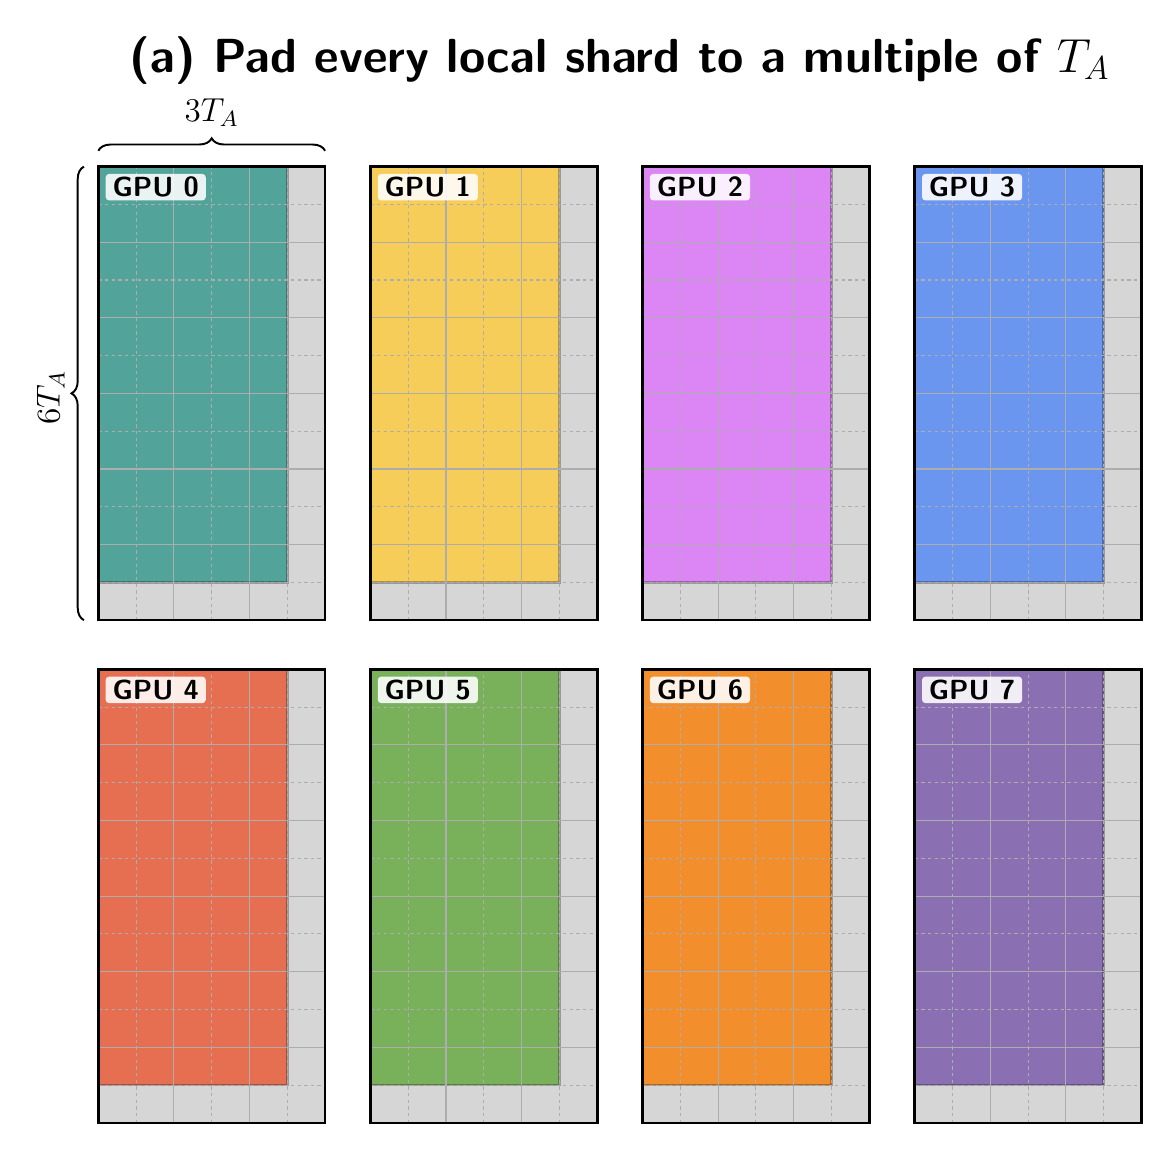
\begin{tikzpicture}[x=.48cm,y=.48cm]
		\node[title] at (13.8,28.1)
		{(a) Pad every local shard to a multiple of $T_A$};

		% Each GPU buffer is 6 x 12:
		% 3 tiles wide and 6 tiles high.
		% With a 2 x 4 GPU grid, the full padded layout is 24 x 24.
		\foreach \r in {0,1}{
			\foreach \c in {0,1,2,3}{
				\pgfmathtruncatemacro{\g}{4*\r+\c}
				\pgfmathsetmacro{\x}{7.2*\c}
				\pgfmathsetmacro{\y}{13.3*(1-\r)}
				\edef\thiscolor{gpu\g}

				% Padding background.
				\fill[padgray] (\x,\y) rectangle ++(6,12);

				% Valid local data region: 5 x 10.

				\fill[\thiscolor]
				(\x,\y+1) rectangle ++(5,11);

				\drawrectshadow
				{\x}{\y+1}{5}{11}


				% Tile guides for T_A = 2.
				\foreach \k in {1,...,5}{
					\draw[guide]
					(\x+\k,\y)--(\x+\k,\y+12);
				}
				\foreach \k in {1,...,11}{
					\draw[guide]
					(\x,\y+\k)--(\x+6,\y+\k);
				}
				\drawlocaltileboundaries{\x}{\y}

				\draw[processor] (\x,\y) rectangle ++(6,12);

				\node[gpulabel,anchor=north west]
				at (\x+.18,\y+11.82) {GPU \g};
			}
		}

		% Dimension annotations on GPU 0.
		\draw[brace] (0,25.72)--(6,25.72)
		node[midway,above=5pt,font=\sffamily\large] {$3T_A$};

		\draw[brace] (-.38,13.3)--(-.38,25.3)
		node[
		midway,
		left=12pt,
		yshift=12pt,
		font=\sffamily\large,
		rotate=90
		] {$6T_A$};
	\end{tikzpicture}
	% =============================================================================
	% Figure 2: column compaction
	% =============================================================================
	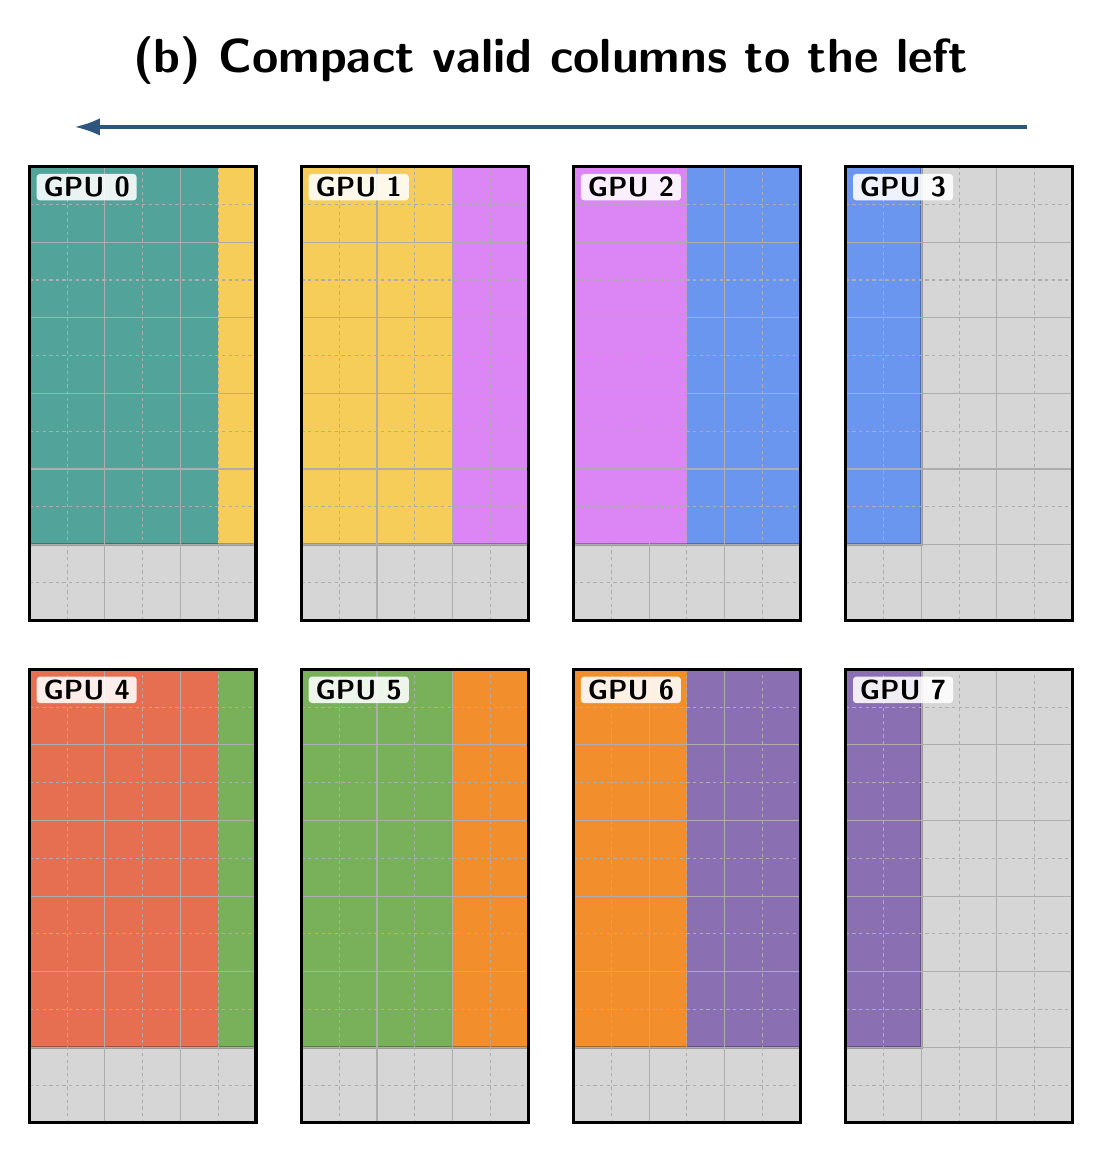
\begin{tikzpicture}[x=.48cm,y=.48cm]
		\node[title] at (13.8,28.1)
		{(b) Compact valid columns to the left};

		% Each GPU buffer is 6 x 12, so the complete 2 x 4 GPU layout
		% represents a square 24 x 24 padded matrix.
		\foreach \r in {0,1}{
			\foreach \c in {0,1,2,3}{
				\pgfmathtruncatemacro{\g}{4*\r+\c}
				\pgfmathsetmacro{\x}{7.2*\c}
				\pgfmathsetmacro{\y}{13.3*(1-\r)}

				% Local padded buffer.
				\fill[padgray] (\x,\y) rectangle ++(6,12);

				% Compact valid columns:
				% GPU columns 0,1,2 receive 6 columns;
				% GPU column 3 receives the remaining 2 columns.
				\foreach \lx in {0,...,5}{
					\pgfmathtruncatemacro{\gx}{6*\c+\lx}

					\ifnum\gx<20\relax
					\pgfmathtruncatemacro{\sourcecol}{int(\gx/5)}
					\pgfmathtruncatemacro{\sourcegpu}{4*\r+\sourcecol}
					\edef\thiscolor{gpu\sourcegpu}

					\fill[\thiscolor]
					(\x+\lx,\y+2) rectangle ++(1,10);
					\fi
				}

				% One shadow around the complete valid region on this GPU.
				\ifnum\c<3\relax
				\drawrectshadow{\x}{\y+2}{6}{10}
				\else
				\drawrectshadow{\x}{\y+2}{2}{10}
				\fi

				% Gray grid lines.
				\foreach \k in {1,...,5}{
					\draw[guide]
					(\x+\k,\y)--(\x+\k,\y+12);
				}
				\foreach \k in {1,...,11}{
					\draw[guide]
					(\x,\y+\k)--(\x+6,\y+\k);
				}
				\drawlocaltileboundaries{\x}{\y}

				\draw[processorboundary]
				(\x,\y) rectangle ++(6,12);

				\node[gpulabel,anchor=north west]
				at (\x+.18,\y+11.82) {GPU \g};
			}
		}

		% Shift arrow for both processor rows.
		\draw[flow] (26.4,26.35)--(1.2,26.35);

	\end{tikzpicture}

	% =============================================================================
	% Figure 3: row compaction
	% =============================================================================
	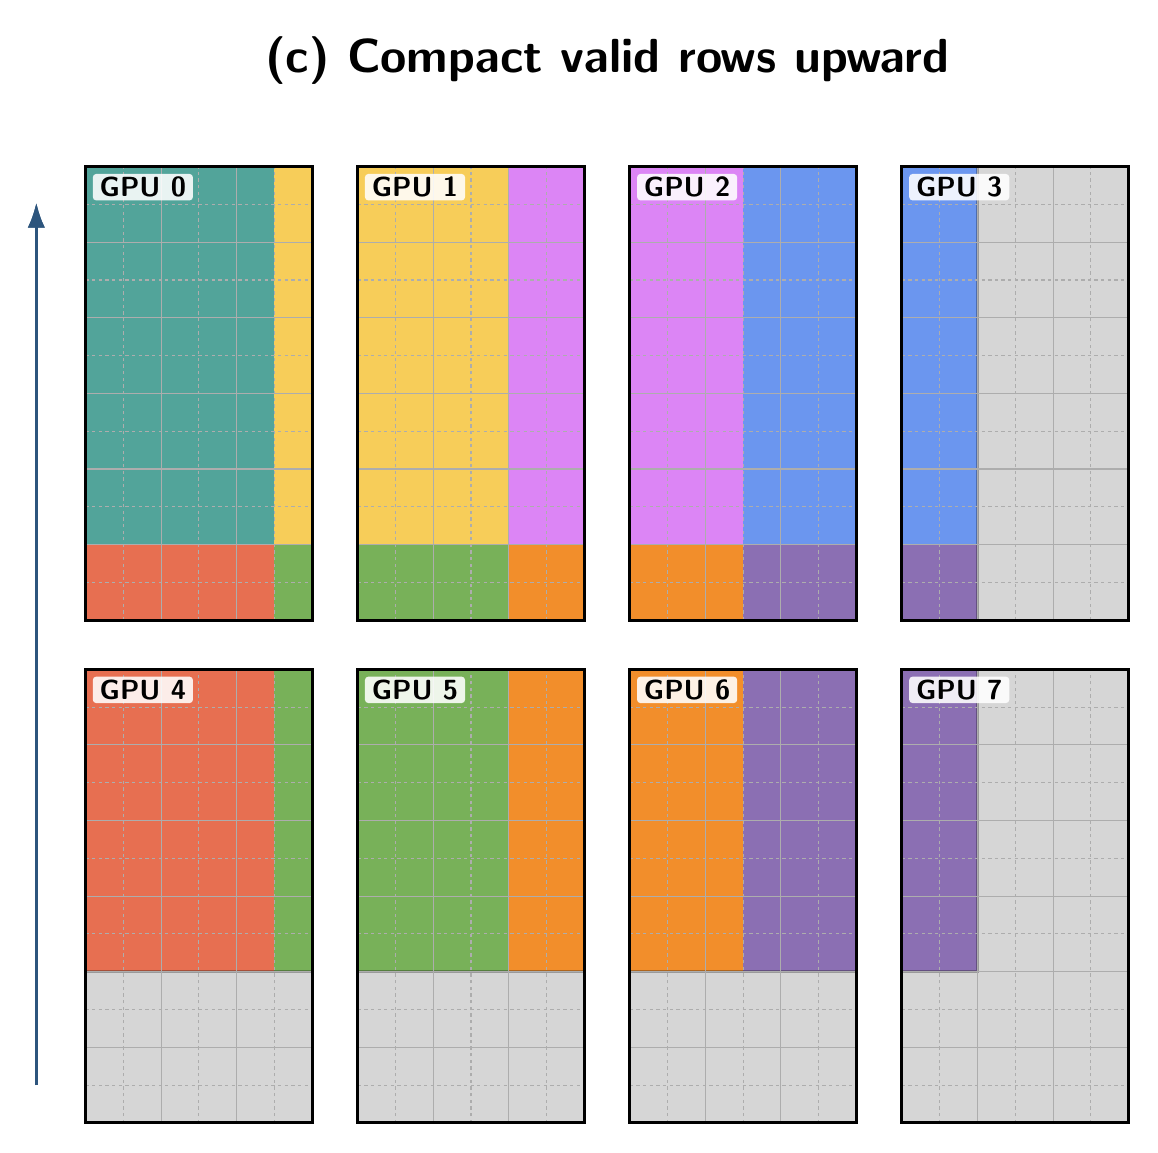
\begin{tikzpicture}[x=.48cm,y=.48cm]
		\node[title] at (13.8,28.1)
		{(c) Compact valid rows upward};

		\foreach \r in {0,1}{
			\foreach \c in {0,1,2,3}{
				\pgfmathtruncatemacro{\g}{4*\r+\c}
				\pgfmathsetmacro{\x}{7.2*\c}
				\pgfmathsetmacro{\y}{13.3*(1-\r)}

				% Local padded buffer.
				\fill[padgray] (\x,\y) rectangle ++(6,12);

				% Draw the globally compacted 20 x 20 data region.
				\foreach \ly in {0,...,11}{
					\foreach \lx in {0,...,5}{
						\pgfmathtruncatemacro{\gx}{6*\c+\lx}
						\pgfmathtruncatemacro{\gy}{12*(1-\r)+\ly}

						\ifnum\gx<20\relax
						\ifnum\gy>3\relax
						\pgfmathtruncatemacro{\sourcecol}
						{int(\gx/5)}

						\ifnum\gy<14\relax
						\pgfmathtruncatemacro{\sourcerow}{1}
						\else
						\pgfmathtruncatemacro{\sourcerow}{0}
						\fi

						\pgfmathtruncatemacro{\sourcegpu}
						{4*\sourcerow+\sourcecol}
						\edef\thiscolor{gpu\sourcegpu}

						\fill[\thiscolor]
						(\x+\lx,\y+\ly) rectangle ++(1,1);
						\fi
						\fi
					}
				}

				% Valid width:
				% first three processor columns are 6 entries wide,
				% final processor column is 2 entries wide.
				\ifnum\c<3\relax
				\def\validwidth{6}
				\else
				\def\validwidth{2}
				\fi

				% Valid height:
				% top processor row is 12 entries high,
				% bottom processor row is 8 entries high.
				\ifnum\r=0\relax
				\pgfmathsetmacro{\validy}{\y}
				\def\validheight{12}
				\else
				\pgfmathsetmacro{\validy}{\y+4}
				\def\validheight{8}
				\fi

				% Shadow around the complete valid region on this GPU.
				\drawrectshadow
				{\x}{\validy}{\validwidth}{\validheight}

				% Gray grid lines, drawn over the colored region and shadow.
				\foreach \k in {1,...,5}{
					\draw[guide]
					(\x+\k,\y)--(\x+\k,\y+12);
				}
				\foreach \k in {1,...,11}{
					\draw[guide]
					(\x,\y+\k)--(\x+6,\y+\k);
				}
				\drawlocaltileboundaries{\x}{\y}

				\draw[processorboundary]
				(\x,\y) rectangle ++(6,12);

				\node[gpulabel,anchor=north west]
				at (\x+.18,\y+11.82) {GPU \g};
			}
			% Shift arrow for both processor rows.
			\draw[flow] (-1.3, 1)--(-1.3, 24.35);
		}
	\end{tikzpicture}
	% =============================================================================
	% Figure 4: colors
	% =============================================================================
	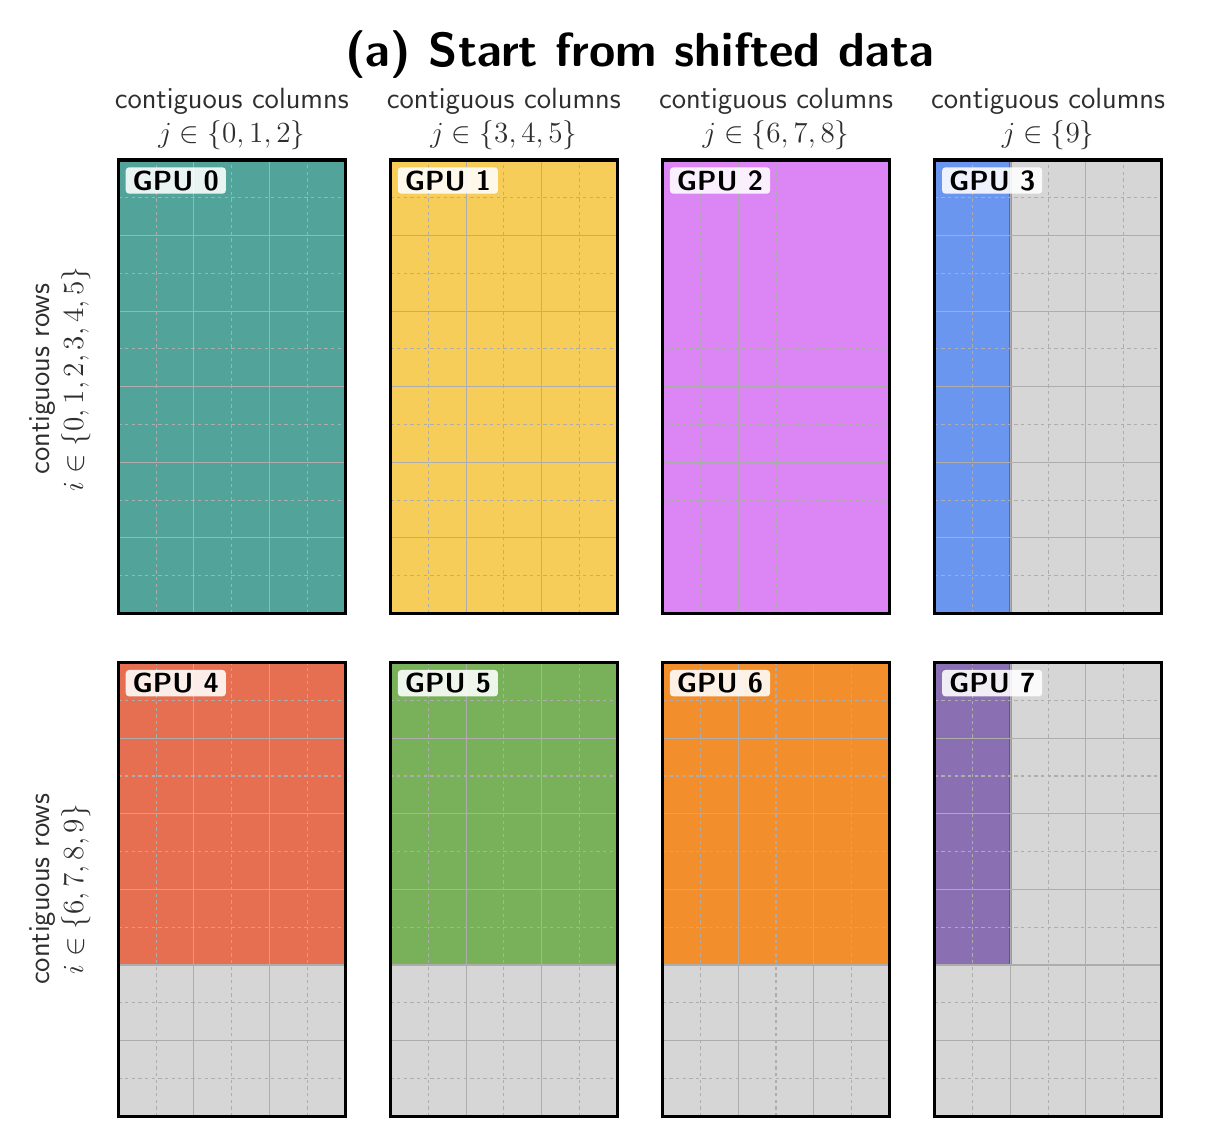
\begin{tikzpicture}[x=.48cm,y=.48cm]
		\path[use as bounding box] (-2.4,-.1) rectangle (28.4,28.8);
		\node[title] at (13.8,28.1)
		{(a) Start from shifted data};

		\foreach \r in {0,1}{
			\foreach \c in {0,1,2,3}{
				\pgfmathtruncatemacro{\g}{4*\r+\c}
				\pgfmathsetmacro{\x}{7.2*\c}
				\pgfmathsetmacro{\y}{13.3*(1-\r)}
				\edef\thiscolor{gpu\g}

				% Local padded GPU buffer.
				\fill[padgray]
				(\x,\y) rectangle ++(6,12);

				% Valid width:
				% GPU columns 0, 1, and 2 contain six columns;
				% GPU column 3 contains the remaining two columns.
				\ifnum\c<3\relax
				\def\validwidth{6}
				\else
				\def\validwidth{2}
				\fi

				% Valid height:
				% the upper GPU row is completely filled;
				% the lower GPU row contains eight rows, aligned at the top.
				\ifnum\r=0\relax
				\pgfmathsetmacro{\validy}{\y}
				\def\validheight{12}
				\else
				\pgfmathsetmacro{\validy}{\y+4}
				\def\validheight{8}
				\fi

				% All valid data currently owned by this GPU receives
				% the color associated with that GPU.
				\fill[\thiscolor]
				(\x,\validy)
				rectangle ++(\validwidth,\validheight);

				% Shadow around the complete valid region.
				\drawrectshadow
				{\x}{\validy}{\validwidth}{\validheight}

				% Entry grid.
				\foreach \k in {1,...,5}{
					\draw[guide]
					(\x+\k,\y)--(\x+\k,\y+12);
				}
				\foreach \k in {1,...,11}{
					\draw[guide]
					(\x,\y+\k)--(\x+6,\y+\k);
				}
				\drawlocaltileboundaries{\x}{\y}

				% GPU-buffer boundary.
				\draw[processorboundary]
				(\x,\y) rectangle ++(6,12);

				\node[gpulabel,anchor=north west]
				at (\x+.18,\y+11.82) {GPU \g};

			}
		}

		% The starting layout owns contiguous block columns and rows.
		\node[note] at (3.0,26.38)
		{contiguous columns\\$j\in\{0,1,2\}$};
		\node[note] at (10.2,26.38)
		{contiguous columns\\$j\in\{3,4,5\}$};
		\node[note] at (17.4,26.38)
		{contiguous columns\\$j\in\{6,7,8\}$};
		\node[note] at (24.6,26.38)
		{contiguous columns\\$j\in\{9\}$};

		\node[note,rotate=90] at (-1.55,19.5)
		{contiguous rows\\$i\in\{0,1,2,3,4,5\}$};
		\node[note,rotate=90] at (-1.55,6.0)
		{contiguous rows\\$i\in\{6,7,8,9\}$};
	\end{tikzpicture}

	% =============================================================================
	% Figure 5: col-cyclic redistribution
	% =============================================================================
	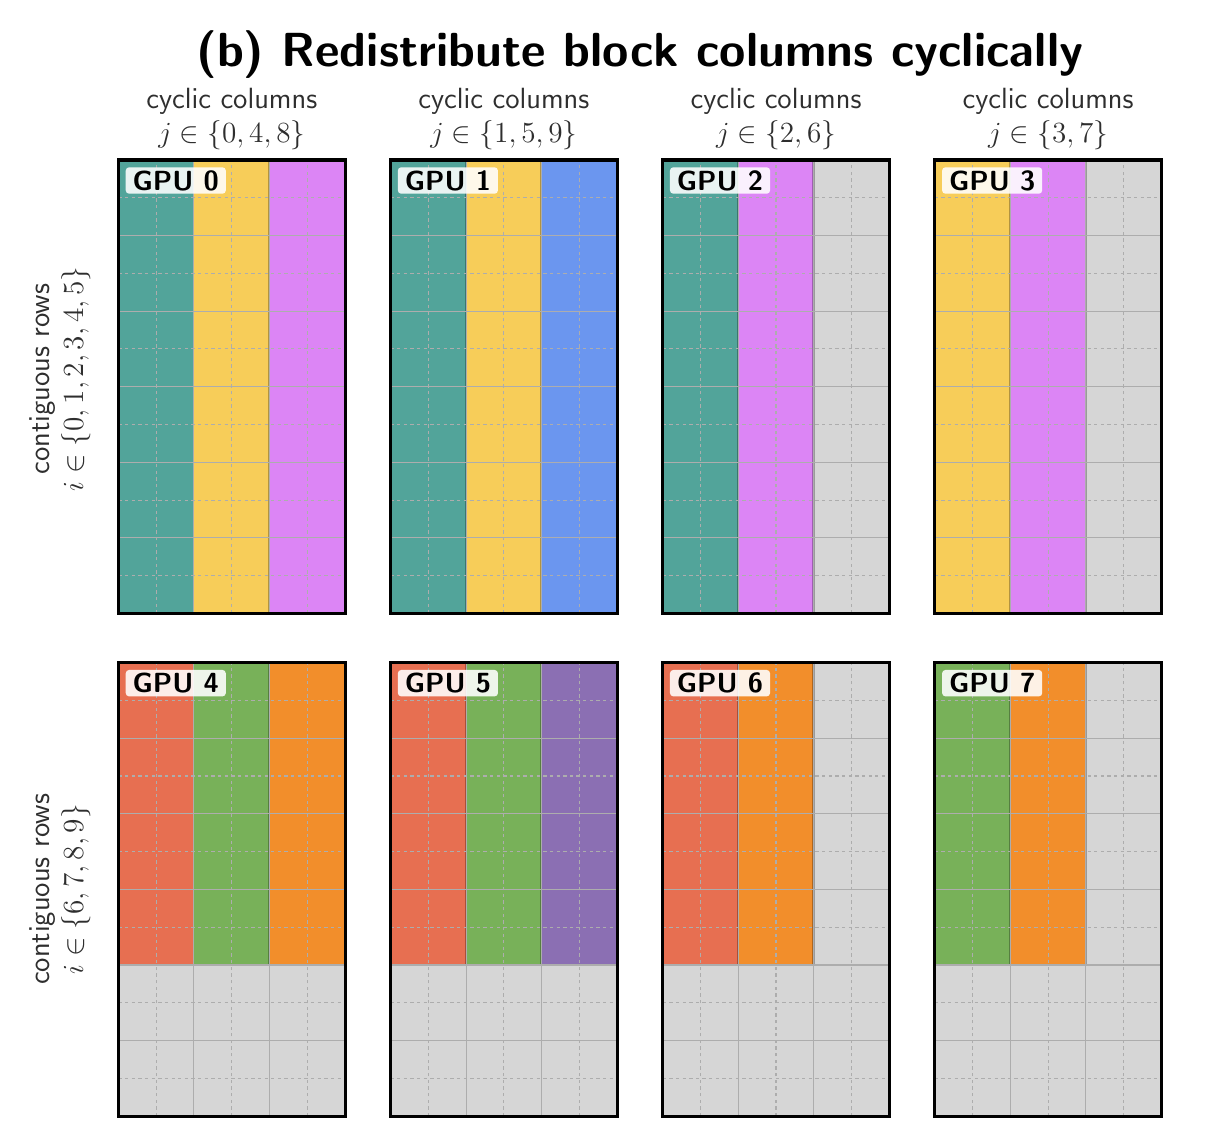
\begin{tikzpicture}[x=.48cm,y=.48cm]
		\path[use as bounding box] (-2.4,-.1) rectangle (28.4,28.8);
		\node[title] at (13.8,28.1)
		{(b) Redistribute block columns cyclically};

		\foreach \r in {0,1}{
			\foreach \c in {0,1,2,3}{
				\pgfmathtruncatemacro{\g}{4*\r+\c}
				\pgfmathsetmacro{\x}{7.2*\c}
				\pgfmathsetmacro{\y}{13.3*(1-\r)}

				% Local padded GPU buffer.
				\fill[padgray]
				(\x,\y) rectangle ++(6,12);

				% The top processor row contains 12 valid entry rows.
				% The bottom processor row contains 8 valid entry rows,
				% aligned with the top of its local buffer.
				\ifnum\r=0\relax
				\pgfmathsetmacro{\validy}{\y}
				\def\validheight{12}
				\else
				\pgfmathsetmacro{\validy}{\y+4}
				\def\validheight{8}
				\fi

				% Destination processor column c receives global block
				% columns j = c, c+4, c+8.
				\foreach \q in {0,1,2}{
					\pgfmathtruncatemacro{\j}{\c+4*\q}

					% Only global block columns j=0,...,9 contain data.
					\ifnum\j<10\relax

					% Before redistribution:
					%   j=0,1,2   came from source processor column 0,
					%   j=3,4,5   came from source processor column 1,
					%   j=6,7,8   came from source processor column 2,
					%   j=9       came from source processor column 3.
					\pgfmathtruncatemacro{\sourcecol}{int(\j/3)}
					\pgfmathtruncatemacro{\sourcegpu}
					{4*\r+\sourcecol}
					\edef\thiscolor{gpu\sourcegpu}

					% Local position of this T_A=2 block column.
					\pgfmathsetmacro{\tilex}{\x+2*\q}

					\fill[\thiscolor]
					(\tilex,\validy)
					rectangle ++(2,\validheight);

					% Give each moved block column its own shadow.
					\drawrectshadow
					{\tilex}{\validy}{2}{\validheight}
					\fi
				}

				% Gray entry grid, drawn above the colored blocks.
				\foreach \k in {1,...,5}{
					\draw[guide]
					(\x+\k,\y)--(\x+\k,\y+12);
				}
				\foreach \k in {1,...,11}{
					\draw[guide]
					(\x,\y+\k)--(\x+6,\y+\k);
				}
				\drawlocaltileboundaries{\x}{\y}

				% Local GPU-buffer boundary.
				\draw[processorboundary]
				(\x,\y) rectangle ++(6,12);

				\node[gpulabel,anchor=north west]
				at (\x+.18,\y+11.82) {GPU \g};
			}
		}

		% Valid global block columns assigned to each processor column.
		\node[note] at (3.0,26.38)
		{cyclic columns\\$j\in\{0,4,8\}$};
		\node[note] at (10.2,26.38)
		{cyclic columns\\$j\in\{1,5,9\}$};
		\node[note] at (17.4,26.38)
		{cyclic columns\\$j\in\{2,6\}$};
		\node[note] at (24.6,26.38)
		{cyclic columns\\$j\in\{3,7\}$};

		% Block rows have not yet been redistributed.
		\node[note, rotate=90] at (-1.55,19.5)
		{contiguous rows\\$i\in\{0,1,2,3,4,5\}$};

		\node[note,rotate=90] at (-1.55,6.0)
		{contiguous rows\\$i\in\{6,7,8,9\}$};
	\end{tikzpicture}
	% =============================================================================
	% Figure 6: final 2D block-cyclic form
	% =============================================================================
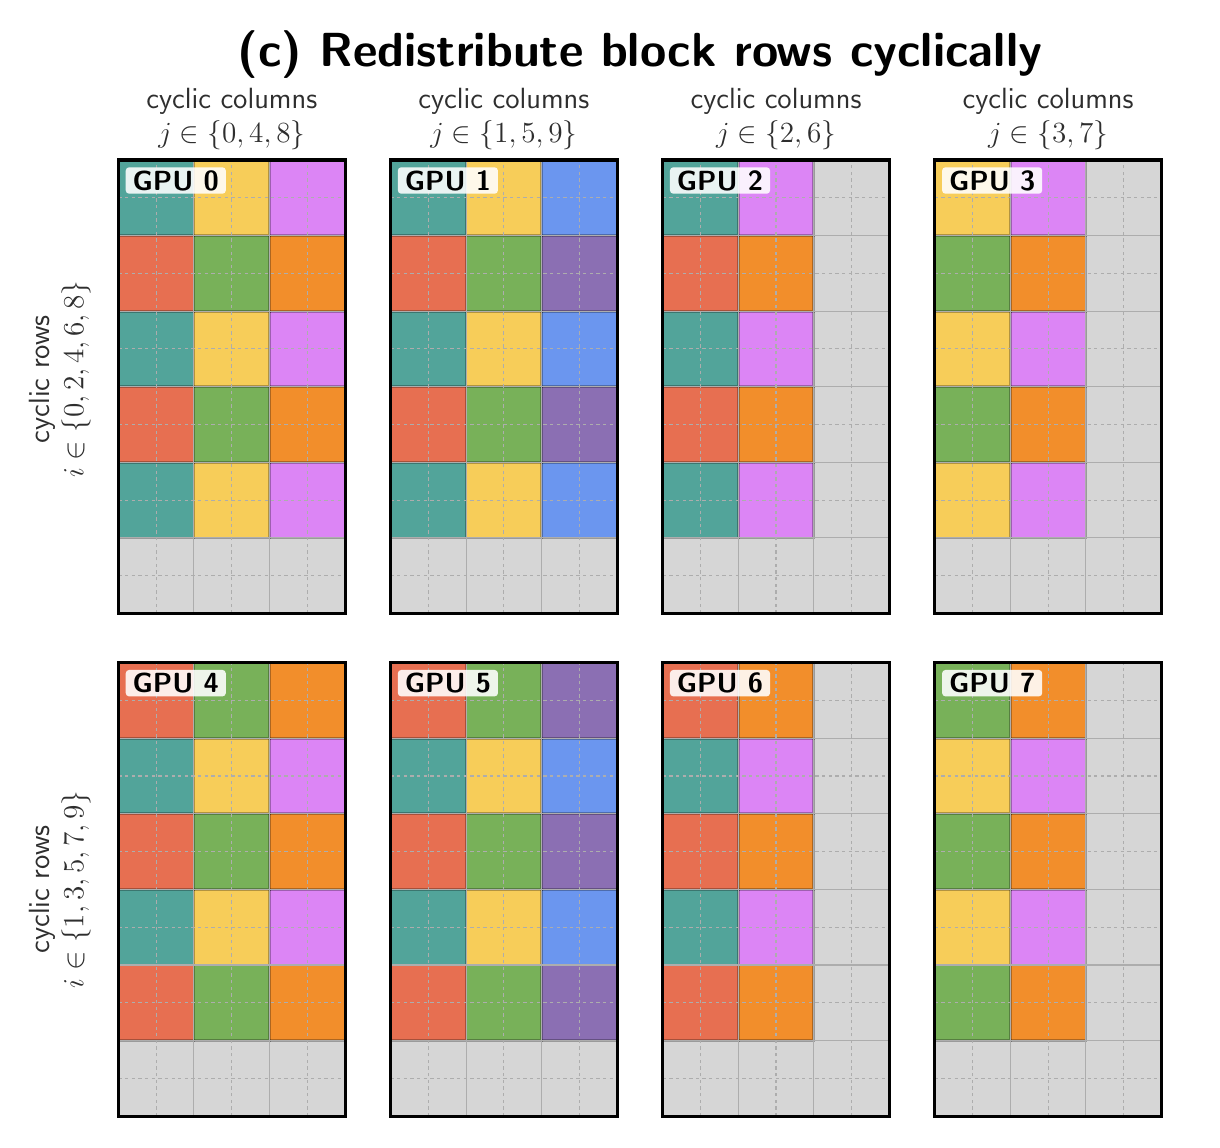
\begin{tikzpicture}[x=.48cm,y=.48cm]
	\path[use as bounding box] (-2.4,-.1) rectangle (28.4,28.8);
	\node[title] at (13.8,28.1)
	{(c) Redistribute block rows cyclically};

	\foreach \r in {0,1}{
		\foreach \c in {0,1,2,3}{
			\pgfmathtruncatemacro{\g}{4*\r+\c}
			\pgfmathsetmacro{\x}{7.2*\c}
			\pgfmathsetmacro{\y}{13.3*(1-\r)}

			% Local padded GPU buffer: 3 x 6 tiles.
			\fill[padgray]
			(\x,\y) rectangle ++(6,12);

			% ---------------------------------------------------------
			% First pass: draw the interwoven T_A x T_A tiles.
			% ---------------------------------------------------------
			\foreach \localtilerow in {0,...,4}{
				\foreach \localtilecol in {0,...,2}{

					\pgfmathtruncatemacro{\i}
					{\r+2*\localtilerow}
					\pgfmathtruncatemacro{\j}
					{\c+4*\localtilecol}

					% Only ten global tile columns are valid.
					\ifnum\j<10\relax

					% Original processor column.
					\pgfmathtruncatemacro{\sourcecol}
					{int(\j/3)}

					% Alternate the source processor row after
					% every T_A-high tile.
					\pgfmathtruncatemacro{\sourcerow}
					{mod(\localtilerow+\r,2)}

					\pgfmathtruncatemacro{\sourcegpu}
					{4*\sourcerow+\sourcecol}
					\edef\thiscolor{gpu\sourcegpu}

					% Five valid tile rows aligned at the top.
					\pgfmathsetmacro{\tilex}
					{\x+2*\localtilecol}
					\pgfmathsetmacro{\tiley}
					{\y+10-2*\localtilerow}

					\fill[\thiscolor]
					(\tilex,\tiley)
					rectangle ++(2,2);
					\fi
				}
			}

			% ---------------------------------------------------------
			% Second pass: shadow each individual T_A x T_A tile.
			% Drawing shadows separately prevents subsequent tile fills
			% from covering the shadows.
			% ---------------------------------------------------------
			\foreach \localtilerow in {0,...,4}{
				\foreach \localtilecol in {0,...,2}{

					\pgfmathtruncatemacro{\j}
					{\c+4*\localtilecol}

					\ifnum\j<10\relax
					\pgfmathsetmacro{\tilex}
					{\x+2*\localtilecol}
					\pgfmathsetmacro{\tiley}
					{\y+10-2*\localtilerow}

					\drawrectshadow
					{\tilex}{\tiley}{2}{2}
					\fi
				}
			}

			% Entry-level gray grid.
			\foreach \k in {1,...,5}{
				\draw[guide]
				(\x+\k,\y)--(\x+\k,\y+12);
			}
			\foreach \k in {1,...,11}{
				\draw[guide]
				(\x,\y+\k)--(\x+6,\y+\k);
			}

			\drawlocaltileboundaries{\x}{\y}

			\draw[processorboundary]
			(\x,\y) rectangle ++(6,12);

			\node[gpulabel,anchor=north west]
			at (\x+.18,\y+11.82) {GPU \g};
		}
	}

	\node[note] at (3.0,26.38)
	{cyclic columns\\$j\in\{0,4,8\}$};
	\node[note] at (10.2,26.38)
	{cyclic columns\\$j\in\{1,5,9\}$};
	\node[note] at (17.4,26.38)
	{cyclic columns\\$j\in\{2,6\}$};
	\node[note] at (24.6,26.38)
	{cyclic columns\\$j\in\{3,7\}$};

	\node[note,rotate=90] at (-1.55,19.5)
	{cyclic rows\\
		$i\in\{0,2,4,6,8\}$};

	\node[note,rotate=90] at (-1.55,6.0)
	{cyclic rows\\
		$i\in\{1,3,5,7,9\}$};
\end{tikzpicture}
\end{document}
